
\documentclass[a4paper, 12pt]{article}

\usepackage{wrapfig}
\usepackage{graphicx}
\usepackage{mathtext}
\usepackage{amsmath}
\usepackage{siunitx}
\usepackage{multirow}
\usepackage{rotating}

\usepackage[T1,T2A]{fontenc}

\usepackage[russian]{babel}

\graphicspath{{pictures/}}

\title{ \begin{center}СИЛА КОРИОЛИСА\end{center}
ОТКЛОНЕНИЕ ПАДАЮЩИХ ТЕЛ ОТ НАПРАВЛЕНИЯ ОТВЕСА}
\author{Иванов И. И.}
\date{\today}

\begin{document}
\maketitle
\newpage
\section{Определение и немного истории}
\paragraph{}
Сила Кориол\'uса — одна из сил инерции ( псевдосила ), возникающая при рассмотрении движения тела во вращающейся системе отсчета. Вычисляется следующим образом: 
\[ F_{кор} = -2m[\overrightarrow{\omega}, \overrightarrow{v_{отн}}]\]
где:
\[ \overrightarrow{v_{отн}} - \text{скорость тела во вращающейся СО,} \qquad \overrightarrow{\omega} - \text{угловая скорость вращения СО}\]
\paragraph{}
Получила имя французского ученого Гасп\'aра-Гюст\'aва де Кориол\'uса, впервые ( как считается ) описавшего её в статье 1835 года. Однако некоторые люди утверждают, что первое математическое выражение для этой силы получил Пьер-Симон Лаплас в 1775 году, а эффект отклонения движущихся объектов во вращающихся системах отсчёта был описан Джованни Баттиста Риччоли и Франческо Мария Гримальди в 1651 году.
\section{Вывод}
\paragraph{}
Расмотрим две системы отсчета: инерциальную $S$ и произвольную $S'$. Пусть $(\overrightarrow{i}, \overrightarrow{j}, \overrightarrow{k}) $- взаимноперпендикулярные единичные базисные векторы системы координат в $S'$, образующие правую тройку. $\overrightarrow{R_0}$ - радиус-вектор начала координат $S'$ в $S$, $\overrightarrow{R}$ - радиус-вектор движущейся точки М в $S$, $\overrightarrow{r}$ - радиус-вектор М в $S'$. Рассмотрим поступательное движение точки М в $S'$, при этом сама система координат $S'$ может двигаться произвольным образом. Тогда ее движение можно разложить на поступательное с некоторой скоростью $\dot{\overrightarrow{R_0}} = \overrightarrow{v_0}$, ускорением $\ddot{\overrightarrow{R_0}} = \dot{\overrightarrow{v_0}}$, и вращательное относительно начала координат с угловой скоростью $\omega$. Тогда найдем $\overrightarrow{v_{абс}}$ скорость и $\overrightarrow{a_{абс}}$ ускорение точки М в $S$, зная соответствующие параметры М $\overrightarrow{v_{отн}}$ и $\overrightarrow{a_{отн}}$ в $S'$:
\[ \overrightarrow{R} = \overrightarrow{R_0} + \overrightarrow{r} = x \overrightarrow{i} + y \overrightarrow{j} + z \overrightarrow{k} + \overrightarrow{R_0}  \]
\[ \overrightarrow{v_{абс}} = \dot{\overrightarrow{R}} + ( \dot{x}\overrightarrow{i} + \dot{y}\overrightarrow{j} + \dot{z}\overrightarrow{k} ) + ( x \dot{\overrightarrow{i}} + y\dot{\overrightarrow{j}} + z\dot{\overrightarrow{k}} )\]
где:
\[ \dot{\overrightarrow{R}} = \overrightarrow{v_0} \qquad
\dot{x}\overrightarrow{i} + \dot{y}\overrightarrow{j} + \dot{z}\overrightarrow{k} = \overrightarrow{v_{отн}}\]
\[ \dot{\overrightarrow{i}} = [\overrightarrow{\omega}, \overrightarrow{i} ] \quad  \dot{\overrightarrow{j}} = [\overrightarrow{\omega}, \overrightarrow{j} ] \quad \dot{\overrightarrow{k}} = [\overrightarrow{\omega}, \overrightarrow{k} ] \quad\]
Имеем:
\[ \overrightarrow{v_{абс}} = \dot{\overrightarrow{R}} + ( \dot{x}\overrightarrow{i} + \dot{y}\overrightarrow{j} + \dot{z}\overrightarrow{k} ) + ( x[\overrightarrow{\omega}, \overrightarrow{i} ] + y[\overrightarrow{\omega}, \overrightarrow{j} ] + z[\overrightarrow{\omega}, \overrightarrow{k} ]  ) = \overrightarrow{v_0} + \overrightarrow{v_{отн}} + [\overrightarrow{\omega}, \overrightarrow{r} ]\]
Тогда:
\[ \overrightarrow{a_{абс}} = \dot{\overrightarrow{v_0}} + 2( \dot{x}\dot{\overrightarrow{i}} + \dot{y}\dot{\overrightarrow{j}} + \dot{z}\dot{\overrightarrow{k}} ) + ( \ddot{x}\overrightarrow{i} + \ddot{y}\overrightarrow{j} + \ddot{z}\overrightarrow{k} ) + ( x \ddot{\overrightarrow{i}} + y\ddot{\overrightarrow{j}} + z\ddot{\overrightarrow{k}} )\]
где:
\[ \ddot{x}\overrightarrow{i} + \ddot{y}\overrightarrow{j} + \ddot{z}\overrightarrow{k} = \overrightarrow{a_{отн}}\]
\[ \dot{x}\dot{\overrightarrow{i}} + \dot{y}\dot{\overrightarrow{j}} + \dot{z}\dot{\overrightarrow{k}} = \dot{x}[\overrightarrow{\omega}, \overrightarrow{i} ] + \dot{y}[\overrightarrow{\omega}, \overrightarrow{j} ] + \dot{z}[\overrightarrow{\omega}, \overrightarrow{k} ] = [\overrightarrow{\omega}, \overrightarrow{v_{отн}}] \]
\[ x\ddot{\overrightarrow{i}} = x[\dot{\overrightarrow{\omega}}, \overrightarrow{i} ] + x[\overrightarrow{\omega}, \dot{\overrightarrow{i}} ] = x[\dot{\overrightarrow{\omega}}, \overrightarrow{i} ] + x[\overrightarrow{\omega}, [\overrightarrow{\omega}, \overrightarrow{i}] ] = [\dot{\overrightarrow{\omega}}, \overrightarrow{r_x} ] + [\overrightarrow{\omega}, [\overrightarrow{\omega}, \overrightarrow{r_x}] ] = \]
\[ = [\dot{\overrightarrow{\omega}}, \overrightarrow{r_x} ] + \overrightarrow{\omega}( \overrightarrow{\omega}, \overrightarrow{r_x}) - \overrightarrow{r_x}( \overrightarrow{\omega}, \overrightarrow{\omega} ) = [\dot{\overrightarrow{\omega}}, \overrightarrow{r_x} ] + \omega^2(\overrightarrow{r_{x\parallel}} - \overrightarrow{r_x} ) = [\dot{\overrightarrow{\omega}}, \overrightarrow{r_x} ] - \omega^2 \overrightarrow{r_{x\perp}}  \]
Окончательно:
\[ \overrightarrow{a_{абс}} = \dot{\overrightarrow{v_0}} + \overrightarrow{a_{отн}} + 2[\overrightarrow{\omega}, \overrightarrow{v_{отн}}] + [\dot{\overrightarrow{\omega}}, \overrightarrow{r}] - \omega^2\overrightarrow{r_{\perp}}\]
Тогда звпишем уравнение, которое можем назвать 2-ым законом Ньютона для неинерциальной системы отсчета $S'$:
\[ m\overrightarrow{a_{отн}} = m\overrightarrow{a_{абс}} - m\dot{\overrightarrow{v_{отн}}} - 2m[\overrightarrow{\omega}, \overrightarrow{v_{отн}}] - m [\dot{\overrightarrow{\omega}}, \overrightarrow{r}] + m\omega^2\overrightarrow{r_{\perp}}\]
где:
\[ m\omega^2\overrightarrow{r_{\perp}} - \text{ центробежная сила,} \qquad -2m[\overrightarrow{\omega}, \overrightarrow{v_{отн}}] - \text{ сила Кориолиса}\]
\section{Пример применения}
\paragraph{}
Рассмотрим влияние силы Кориолиса на движение падающего тела в гравитационном поле Земли ( сопротивлением воздуха пренебрежем ). Рассматривать движение будем в системе отсчета Земли. Ось $z$ направим так, чтобы $\overrightarrow{g} \uparrow \downarrow \overrightarrow{k}$. Ось $x$ возьмем перпендикулярной оси $z$ в плоскости меридиана ( см. рисунок 1 ). Тогда запишем 2-ой закон Ньютона для падающего тела в нашей СО:
\[ \frac{m d\overrightarrow{v}}{dt} = \overrightarrow{mg} + \overrightarrow{F_{кор}}\]
\newpage
\begin{figure}[h]

\centering

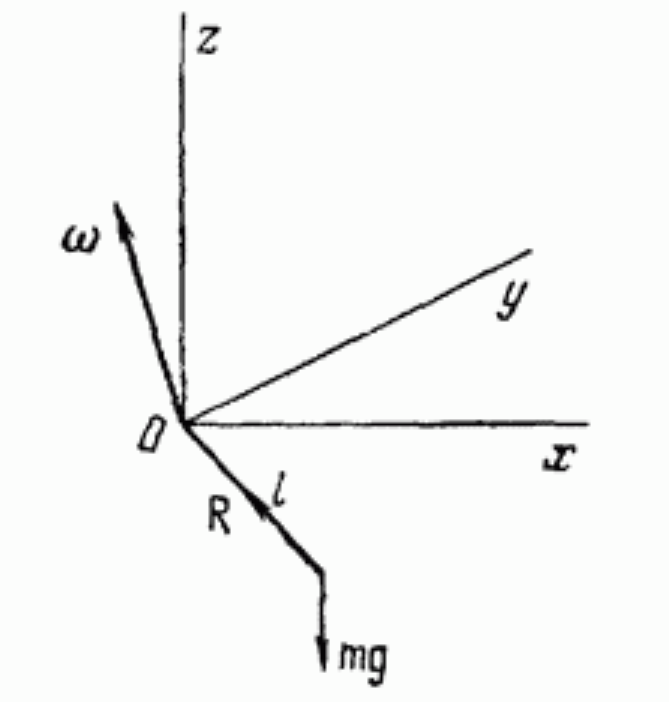
\includegraphics[width=0.4\linewidth]{Koriolis.png}

\caption{Чертеж к задаче о падении точки}

\label{fig:mpr}

\end{figure}
Спроецируем на оси ( $\Omega$- угловая скорость вращения Земли, $\varphi$ - широта, в области которой падает тело ):
\[ OX: \frac{m d^2 x}{dt^2} = 2m \frac{dy}{dt} \Omega sin\varphi\]
\[ OY: \frac{m d^2 y}{dt^2} = - 2m\Omega ( \frac{dx}{dt} sin\varphi + \frac{dz}{dt} cos\varphi)\]
\[ OZ: \frac{m d^2 z}{dt^2} = 2m \frac{dy}{dt} \Omega cos\varphi - mg\] 
Нас интересует частное решение данной системы при следующих начальных условиях:
\[ x(0) = y(0) = z(0) = 0 \qquad
\dot{x}(0) = \dot{y}(0) = \dot{z}(0) = 0\]
Поэтому воспользуемся методом последовательных приближений Пикара. Приведем дифференциальные уравнения к интегральным (*) для удобства:
\[ x(t) = 2\Omega sin\varphi \int_0^t y\,\mathrm{d}t \]
\[ y(t) = -2\Omega sin\varphi \int_0^t x\,\mathrm{d}t -2\Omega cos\varphi \int_0^t z\,\mathrm{d}t \]
\[ z(t) = 2\Omega cos\varphi \int_0^t y\,\mathrm{d}t - \frac{g t^2}{2} \]
Согласно методу каждое следующее приближение выражается через предыдущее формулой: 
\[ x_{n}(t) = 2\Omega sin\varphi \int_0^t y_{n-1}\,\mathrm{d}t \]
\[ y_{n}(t) = -2\Omega sin\varphi \int_0^t x_{n-1}\,\mathrm{d}t -2\Omega cos\varphi \int_0^t z_{n-1}\,\mathrm{d}t \]
\[ z_{n}(t) = 2\Omega cos\varphi \int_0^t y_{n-1}\,\mathrm{d}t - \frac{g t^2}{2} \]
За нулевое приближение берем систему $x_0(t) = y_0(t) = z_0(t) = 0$. Подставляем эти функции в правую часть уравнений (*) и, интегрируя, получаем первое приближение ( соответствует случаю, когда действием силы Кориолиса пренебрегают ):
\[ x_1(t) = y_1(t) = 0 \quad z_1(t) = -\frac{gt^2}{2}\]
Вновь подставляем полученные значения координат в правые части уравнений и интегрируем. Получаем второе приближение ( действие силы Кориолиса учитывается только вдоль оси OY ):
\[ x_2(t) = 0 \quad y_2(t) = \frac{\Omega g t^3 cos\varphi}{3} \quad z_2(t) = -\frac{g t^2}{2}\]
Наконец, третья и последняя итерация:
\[ x_3(t)= \frac{gt^4 \Omega^2 sin\varphi cos\varphi}{4} \quad 
y_3(t) = \frac{gt^3 \Omega cos\varphi}{3} \quad
z_3(t)= \frac{gt^4 \Omega^2 cos^2\varphi - 3 gt^2 }{6}\]
Из полученного решения видно, что тело будет отклоняться в сторону юго-востока. Так, за $t = 10$ с ( широта Москвы $\varphi \approx 55^{\circ}$ ) оно пройдет $x = 0.06$ мм ( южное направление ), $y = 14$ см ( восточное направление ).

\paragraph{}
\emph{Использованная литература:}
\begin{itemize}
    \item Березкин Е.Н. Курс теоретической механики. М.: МГУ, 1974. - 647 с.
    \item Сивухин Д.В. Общий курс физики: Учеб. пособие для вузов. В 5 т. Т. 1. Механика. - 5-е изд., стереот. - М.: ФИЗМАТЛИТ, 2006. - 560 с.
    \item Фрейман Л. С. К истории доказательства теоремы Кориолиса // Труды института истории естествознания и техники / Гл. ред. Н. А. Фигуровский. — М.: АН СССР, 1956. — Т. 10. — С. 213—244.
\end{itemize}
\end{document}
